\section{Methodology Procedure}

\begin{figure}[!htbp]
    \centering
    \centerline{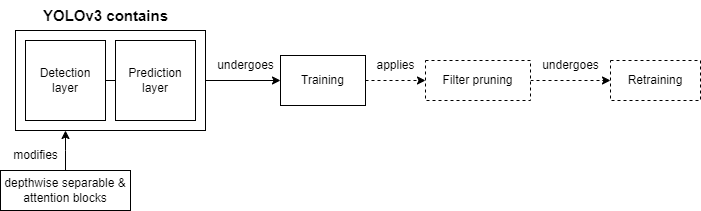
\includegraphics[width=0.95\linewidth]{images/Diagram.png}}
    \caption{Diagram of implementation}
    \label{fig:diagram}
\end{figure}

Figure \ref{fig:diagram} presents the flow to the implementation of the techniques utilized in the study. The broken line arrows and boxes signify additional techniques that may or may not be used by other model variants.

The baseline and every subsequent YOLOv3 implementation followed the Pytorch implementation of Aladdin Persson that is available on Github \cite{MachineLearningCollectionMLPytorch}. 

Each model variant replaced every convolutional layers except for the detection layers \cite{chakarDepthwiseSeparableConvolutions2020}. In addition to this, the modified convolution layers were fused with an attention block \cite{sunYoloBasedLightweightObject2023}. Using the COCO 2017 dataset, the models were trained for 50 epochs, with any additional notes taken regarding the respective models' runtime and metrics generated.

The models were first trained on the COCO dataset and then performed object detection on the MOT17-02-SDP and MOT17-04-SDP sequences, where the average FPS and inference time were recorded. The L1-norm scores for each filter in each layer of the trained model were computed and sorted. Once the L1-norm scores are sorted by value, around 30\% of the weights were pruned from the models. Pruning was done by zeroing the values of the weights. To compensate for this, the parameter count computed all the non-zeroed parameters. The models underwent retraining for the same number of epochs it takes for the baseline model to achieve a minimum 2\% difference in accuracy compared to its unpruned counterpart \cite{liPruningFiltersEfficient2017}. Further performance on the model was noted and compared for evaluation and analysis. 

\begin{table}[!htbp]
    \centering
    \caption{YOLO framework models}
    % \resizebox{0.70\linewidth}{!}
    {
    \begin{tabular}{cc}
        Model & Modifications \\ \hline 
        1& Baseline\\ 
        \hline 
        % 2& Baseline + filter pruning\\ 
        % \hline 
        2&Baseline + CBAM (YOLO-BAM)\\ 
        \hline 
        % 4&Baseline + CBAM + filter pruning\\
        % \hline
        3& Depthwise separable convolutions (DSC)\\
        \hline
        % 6& DSC + Filter pruning \\
        % \hline
        4& DSC + CBAM (DSCBAM)\\
        \hline
        % 8& DSC + CBAM + Filter pruning\\ \hline
    \end{tabular}
    }
    \label{tab:modelvars}
\end{table}

 Table \ref{tab:modelvars} presents the planned model variants and names, where the respective performance of each model such as accuracy and loss were listed down. The additional pruned model variants were also observed and compared to its unpruned versions.
 
In utilizing publicly available datasets for pedestrian detection, it is essential to emphasize that the models developed in this study were not designed to extract individual features for the purpose of identifying specific individuals. Instead, the focus was on modifying the YOLOv3 network for detecting pedestrians in surveillance scenarios. The study aimed to mitigate potential privacy risks by ensuring that any personally identifiable information that can indicate and identify specific individuals was removed during data collection. Additionally, the models were designed to prioritize the detection of generalized pedestrian shapes rather than individual features, further aligning with ethical considerations regarding privacy and personal identification.

\subsection{Statistical Analysis}
To enable a deeper understanding of the performance of the model variants, they will be evaluated with 10 sets of 10 test images for each category, totaling 400 unique images. Once the accuracies are generated, they will then be compared to the baseline YOLOv3 model using a paired two-tailed t-test, where the null and alternative hypotheses are:
\[H_{0} \text{ :  The models' performance is the same.}\] 
\[H_{\alpha} \text{ :  The models' performance is different.}\] 
The variants will be compared with each category to identify those that may be further investigated for future studies. The p-values generated from the t-test will be used to compare against the 95\% confidence interval (alpha = 0.05) to determine if the null hypothesis should be rejected.